\section{Alternative: leader-based approaches}
\label{compaction:leader}

The log compaction approaches presented in this chapter depart from Raft's
strong leader principle, since servers compact their logs without the
knowledge of the leader. However, we think this departure is justified.
While having a leader helps avoid conflicting decisions in reaching
consensus, consensus has already been reached when snapshotting, so no
decisions conflict. Data still only flows from leaders to followers,
but followers can now reorganize their data independently.

We also considered leader-based approaches to log compaction, but any
benefits are usually outweighed by performance considerations.
It would be wasteful for the leader to compact its log, then send the result
to the followers, when they could just as well compact their own logs
independently.
Sending the redundant state to each follower would waste network
bandwidth and slow the compaction process. Each follower already has the
information needed to compact its own state, and the leader's outbound
network bandwidth is usually Raft's most precious (bottleneck) resource.
For memory-based snapshots, it is typically much cheaper for a server to
produce a snapshot from its local state than it is to send and receive
one over the network. For incremental compaction approaches, this depends
a bit more on the hardware configuration, but we also expect independent
compaction to be cheaper.

\subsection{Storing snapshots in the log}

\begin{figure}
\centering
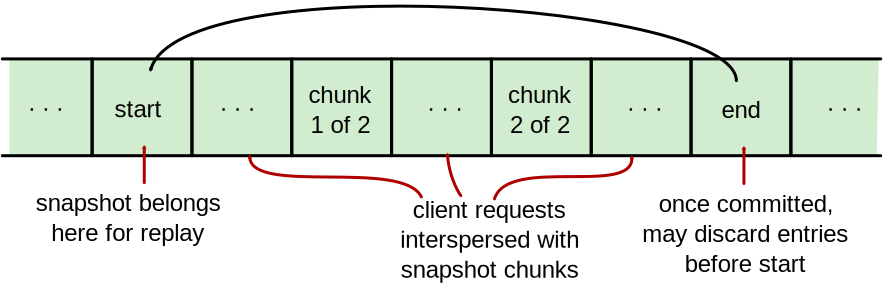
\includegraphics[scale=0.5]{compaction/logbased}
\vcaption[alternative: snapshot stored in log]{
A leader-based approach that stores the snapshot in chunks in the log,
interleaved with client requests. The snapshotting process is started at
the \emph{start} entry, and it completes by the \emph{end} entry.
The snapshot is stored in several log entries between \emph{start} and
\emph{end}.
%
So that client requests can proceed in parallel with snapshotting, each
entry is limited in size, and the rate at which the entries are appended
to the log is limited: the next snapshot chunk is only appended to the
log when the leader learns that the previous snapshot chunk has been
committed.
%
Once each server learns that the \emph{end} entry is committed, it can
discard the entries in its log up to the corresponding \emph{start}
entry. Replaying the log requires a two pass algorithm: the last
complete snapshot is applied first, then the client requests after the
snapshot's \emph{start} entry are applied.
}
\label{fig:compaction:logbased}
\end{figure}

One possible benefit to leader-based approaches is that, if all the
system state could be stored in the log, then new mechanisms to
replicate and persist the state would not be needed. Thus, we considered
a leader-based approach to snapshotting in which the leader would create
a snapshot and store the snapshot as entries in the Raft log, as shown
in Figure~\ref{fig:compaction:logbased}. The leader would then send this
snapshot to each of its followers using the AppendEntries RPC. 
To reduce any disruption on normal operation, each snapshot would be
split into many entries and interleaved with normal client commands in
the log.

This would achieve better economy of mechanism than storing the snapshot
outside the log, since servers would not need separate mechanisms to
transfer snapshots or persist them (they would be replicated and persisted
just like other log entries). However, in addition to wasting network
bandwidth for followers that could just as easily produce their own
snapshots, this has a serious problem. If a leader fails in the middle
of creating a snapshot, it leaves a partial snapshot in the servers'
logs. In principle this could happen repeatedly and exhaust servers'
storage capacity with garbage accumulated from numerous failed
snapshotting attempts. Thus, we don't think this mechanism is viable in
practice.



\subsection{Leader-based approach for very small state machines}

For very small state machines, storing the snapshot in the log not only
becomes viable but can also be simplified significantly. If the snapshot
is small enough (up to about one megabyte), it can fit comfortably in a
single log entry without interrupting normal operation for too long. To
compact the servers' logs in this way, the leader would:
\vspace{2ex}
\begin{compactenum}
\item Stop accepting new client requests;
\item Wait for all entries in its log to be committed and its state
machine to have applied all entries in its log;
\item Take a snapshot (synchronously);
\item Append the snapshot into a single log entry at the end of its log; and
\item Resume accepting new client requests.
\end{compactenum}
Once each server learned that the snapshot entry was committed, it could
discard every entry before the snapshot in its log. This approach would
cause a small availability gap while client requests were stopped and the
snapshot entry was transferred, but its impact would be limited for very
small state machines.

This simpler approach avoids
the implementation effort of persisting snapshots outside the log,
transferring them using a new RPC, and snapshotting concurrently.
However, successful systems tend to be used more than their original
designers intended, and this approach would not work well for larger
state machines.
